%%%%%%%%%%%%%%%%%%%%%%preface.tex%%%%%%%%%%%%%%%%%%%%%%%%%%%%%%%%%%%%%%%%%
% sample preface
%
% Use this file as a template for your own input.
%
%%%%%%%%%%%%%%%%%%%%%%%% Springer %%%%%%%%%%%%%%%%%%%%%%%%%%

\preface

%% Please write your preface here
% Use the template \emph{preface.tex} together with the Springer document class SVMono (monograph-type books) or SVMult (edited books) to style your preface in the Springer layout.

% A preface\index{preface} is a book's preliminary statement, usually written by the \textit{author or editor} of a work, which states its origin, scope, purpose, plan, and intended audience, and which sometimes includes afterthoughts and acknowledgments of assistance. 

% When written by a person other than the author, it is called a foreword. The preface or foreword is distinct from the introduction, which deals with the subject of the work.

% Customarily \textit{acknowledgments} are included as last part of the preface.

\paragraph{Origin}

The reader will find in this monograph a series of tutorials and advanced topics originally written over the last ten years as documentation parts for the \Digraph collection of Python modules. These programming resources -- like the \texttt{outrankingDigraphs} module -- were essentially used for the preparation and illustration of the \emph{Algoritmic Decision Theory} Course taught at the University of Luxembourg from 2010-2020. Some resources, like the \texttt{randomNumbers} module, served as well for preparing and illustrating the Lectures of a \emph{Computational Statistics} Course. Curious readers will also discover some resources --the \texttt{arithmetics} module-- used for preparing and illustrating a first Semester Course on Discrete Mathematics.

\paragraph{Scope}

The \Digraph Python programming resources are useful in the field of \emph{Algorithmic Decision Theory} and more specifically for the outranking approach of \emph{Multiple Criteria Decision Aid} (MCDA). In this latter scientific filed, we address essentially three kinds of usage.
\begin{enumerate}[nosep]
\item First, we present methods an illustrate computing tools for solving either a multiple criteria best choice selection or a dual worst choice rejection problem, mainly interesting for management or social choice studies.
\item We also address the problem of how to list a set of items with multiple incommensurable performance criteria either from the best to the worst (ranking problem) or from the worst to the best (ordering problem), mainly interesting for schedulers or designers of recommender systems.
\item The third kind of usage should mainly be of interest for performance auditors, as we present methods and tools for relative or absolute quantiles rating of mulitiple criteria performance records. 
\end{enumerate}

It is necessary to mention that the \Digraph ressources do not provide a professional Python software library. The collection of Python modules, we describe in this book, was not built following any professional software development methodology. The design of classes and methods was kept as simple and elementary as was opportune for the author. Sophisticated and criptic overloading of classes, methods and variables is more or less avoided all over. A simple copy, paste and ad hoc customization development strategy was generally preferred. As a consequence, the \Digraph modules keep a large part of independence and are hence easier to maintain and adapt.  Furthermore, the development of the \Digraph modules being spread over a decade, our programming style did evolve with our growing experience and the changes and enhancement coming up with the ongoing new releases of the standard Python3 libraries. The required backward compatibility necessarily introduced so with time some notation and programming technique changes.

\paragraph{Plan}

\noindent The book is organized into five parts. Part I presents three chapters introducing the \Digraph resources and the main formal objects discussed in this book, namely \emph{bipolar-valued digraphs} and, in particular, \emph{outranking digraphs}.

Part II illustrates in eight chapters decision methods and tools and performance evaluation models. These methodological chapters are mostly problem oriented and show how to build a best choice recommendation or compute the winner of an election. Others show how to linearly rank or order incommensurable multiple criteria performance records. We also show how to rate such performance records with order-statistical quantiles.

Part III, with four chapters, presents three case studies: --one for building a best choice recommendation for selecting a study program, --one for ranking world famous Computer Science Dpts, and --a third one for rating the student recruitment quality of German Universities. The three case studies are followed by a set of exercises suitable for a Course on Algorithmic Decision Theory.

Part IV presents in five chapters more advanced topics showing some pearls of bipolar-valued epistemic logic. We first generalize \Kendall 's ordinal correlation index to bipolar-valued digraphs in order to measure the fitness of our ranking results. A second and important advanced topic concerns the effective computation of digraph kernels and solving of \Berge kernel equation systems. We furthermore introduce confidence levels for outranking situations when facing uncertain criteria significance weights. And, we develop a robustness analysis of the outranking digraph when facing only ordinal criteria significance weights. The last topic concerns the tempering of plurality tyranny effects in social choice problems with the help a.o. of bipolar approval voting. 

Part V, with three chapters, concerns eventually simple undirected graphs and illustrates operational resources for working with such graphs, like \emph{q-coloring}, enumerating\emph{ maximal independent sets} (MISs) and \emph{cliques}, computing \emph{maximal matchings}, simulating \emph{Metropolis random walks} and enumerating the \emph{non-isomorphic} MISs of the $n$-cycle graph. A second chapter is more specifically devoted to \emph{tree graphs} and \emph{graph forests}. A very last chapter, inspired by Martin Golumbic ‘s book on \emph{Algorithmic Graph Theory and Perfect Graphs}, introduces \emph{split}, \emph{interval} and \emph{permutation} graphs.

\paragraph{Intended audience}

The material in this book is valuable for master students and doctoral candidates in Computer Science, Mathematics, Engineering Sciences or Computational Management Sciences taking a course on Algorithmic Decision Theory, Multiple criteria Decision Aid or Decision Analysis. Some experience in computer programming, in particular with Python, is certainly easing the lecture, but it is not a prerequisite. The many coding examples shown all over the text are kept on purpose very elementary from a programming point of view. 

The chapters where we present methods and tools for ranking multiple criteria performance records from best to worst --especially when facing big performance tableaux-- may be of interest for designers of web recommender systems. 

Similarly, the relative and absolute quantiles rating methods and tools we discuss and illustrate might be of practical interest for private or public performance auditors.

Finally, we do not provide any mathematical developments or proofs. Readers, interested in the mathematical background of our decision methods and tools, are invited to consult the references provided at chapter level. Full texts of most of these references may be downloaded from the \href{https://orbilu.uni.lu/}{https://orbilu.uni.lu/} repository of the University of Luxembourg. 

\paragraph{Aknowledgments}

This mongraph contains many ideas, methods and tools that are not only the author’s. They have been shared and enhanced with friends and colleagues: 

\vspace{0.5cm}
\begin{minipage}{7cm}
\emph{Denis Bouyssou, Luis Dias,}\\ 
\emph{Claude Lamboray, Patrick Meyer,}\\
\emph{Vincent Mousseau, Alex Olteanu,}\\
\emph{Marc Pirlot, late Bernard Roy,}\\
\emph{Alexis Tsouki\`as, Thomas Veneziano,}\\
and especially,\\
\emph{late Marc Roubens}.
\end{minipage}\quad
\begin{minipage}{3cm}
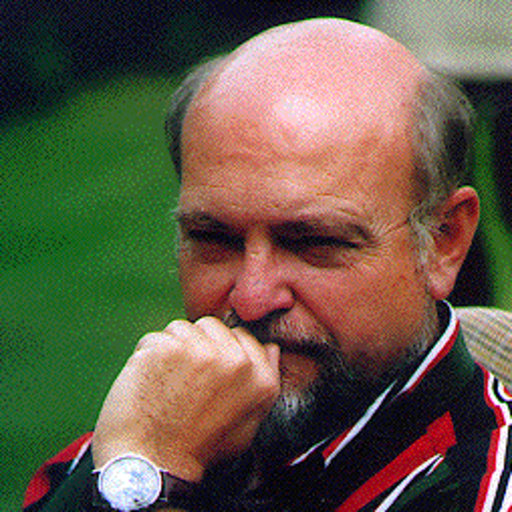
\includegraphics[width=3cm]{Figures/Marc-Roubens.jpg} \\
{\tiny \emph{Marc Roubens}}
\end{minipage}

\vspace{0.3cm}
Their help is gratefully acknowledged.

\vspace{\baselineskip}
\begin{flushright}\noindent
Luxembourg, 2021\hfill {\it Raymond Bisdorff}\\
%month year\hfill {\it Firstname  Surname}\\
\end{flushright}


